
\begin{center}
	\textbf{Schüler haben's schwer \punkte\footcite{prepolino2010}}\\
\end{center}


\begin{figure}[h]
	\centering
		
\includegraphics[width=0.4\textwidth]{images/Lasten-eines-Schuelers.jpg}\\
	\caption{Lasten eines Schülers}
	\label{fig:Lasten-eines-Schuelers}
\end{figure}

\vspace*{\fill}

\begin{center}
	\textbf{\punkte\ Lehrer aber auch\footcite{prepolino2010}}\\
\end{center}


\begin{figure}[h]
	\centering
		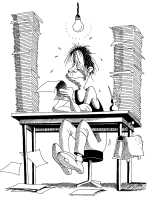
\includegraphics[width=0.4\textwidth]{images/Lasten-eines-Lehrers.jpg}\\
	\caption{Lasten eines Lehrers}
	\label{fig:Lasten-eines-Lehrers}
\end{figure}





